\section{Transmission de données}
\label{TDD}
	\subsection{Protocoles de liaison}
		Le protocole définit le format de la trame avec de bit de controles:
		\begin{itemize}
			\item Source/dest
			\item Etablissement de la liaison
			\item Gestion de l'acces
			\item \dots
		\end{itemize}
		
		Certains role important :
		\begin{itemize}
			\item Medium acces control (MAC)
			\begin{itemize}
				\item Gere le multiplexage entre utilisateur du lien PHY
				\item centralisé ou distribué
				\item ex : 4G/GSM/LTE/\dots
			\end{itemize}
			\item Firward Error Correction (FEC)
			\begin{itemize}
				\item Codes correcteurs d'erreurs
			\end{itemize}
			\item Automatic Repeat Request  (ARQ)
			\begin{itemize}
				\item Mécanisme de retransmition 
			\end{itemize}
		\end{itemize}
		
	\subsection{MAC : Multiplexage}
		\subsubsection{Frequency Domain Multiple Access (FDMA)}

			Principe des différentes radio FM : Chaque radio a une place en fréquence attribuée, Utilisé pour répartir plusieur utilisateurs dans un systeme
			\begin{figure}[htp]
				\centering
				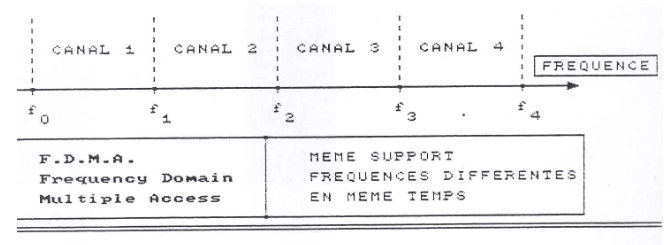
\includegraphics[width=0.7\textwidth]{img/FDMA.png}
			\end{figure}
		
		\subsubsection{Time Domain Multiple Access (TDMA)}
			Meme principe que FDMA
			
			Definitions d'une période de temps qui va se répéter et  qui est diviése en timeslots TDMA. Un timeslot est attribuée a un utilisateur et ne poura envoyer que pendant le timeslot asssigné a chaque période répétitives.
			
			\begin{figure}[htp]
				\centering
				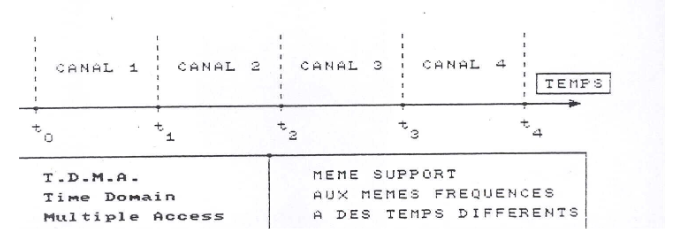
\includegraphics[width=0.7\textwidth]{img/TDMA.png}
				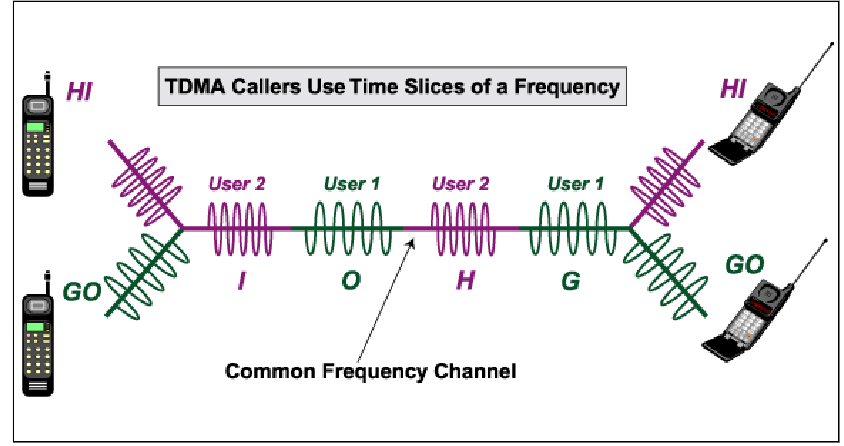
\includegraphics[width=0.7\textwidth]{img/TDMA1.png}
			\end{figure}
		\subsubsection{Code Division Multiple Access (CDMA)}
		
			Pour diviser les utilisateurs  on utilise plus le temps ou la fréquence mais un code (comme pour le 3G)
			
			Contient 3 signaux:
			\begin{itemize}
				\item \textbf{Data Signal :} Signal binaire composé d'une période $T_b$ (durée d'un bit d'info envoyé)
				\item \textbf{PseudoRandom Code :} Code spécifique à chaque utilisateur permettant d'encoder/moduler le data signal
				
				La durée du \textit{Chip} ($T_c < T_b$)
				\item \textbf{Transmitted signal} : Signal transmit qui est le resultat d'un application XOR avec le \textbf{Data signal} et \textit{PseudoRandom Code}
			\end{itemize}
			
			\begin{figure}[htp]
				\centering
				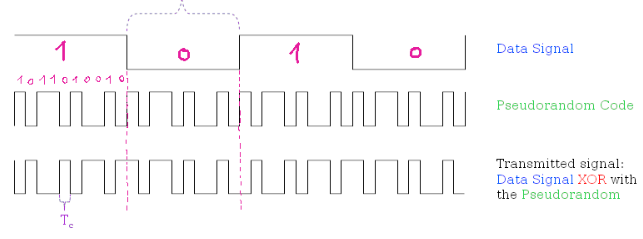
\includegraphics[width=0.7\textwidth]{img/CDMA.png}
			\end{figure}
			
	\subsection{Gestion des erreurs}
		\subsubsection{Causes des erreurs}
			\begin{itemize}
				\item Dispersion dans les lignes
				\item Bruit thermique
				\item Bruit Impulsif
				\item Echos/diaphonie
				\item Perte de synchro
				\item Effet "amplifiés" en fonction de l'atténuations
			\end{itemize}
			
		\subsubsection{Code détecteur et correcteur d'erreur}
		
			Principe de base : envoyer de le redondance
			
			\textbf{Ex1:} Code de parité :
				
				Verifier si le nombre de bits est paire ou impaire pour chaque période d'envois
				
				Limité si on on a des erreurs doubles dans le meme bloc
				
				\begin{figure}[htp]
					\centering
					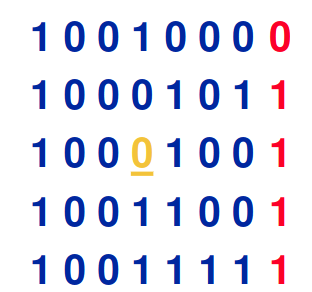
\includegraphics[width=0.3\textwidth]{img/Erreur.png}
				\end{figure}
				
			\newpage
				
			\textbf{Ex2 :} Langues/dictionnaire de mots valables
			
			\begin{figure}[htp]
				\centering
				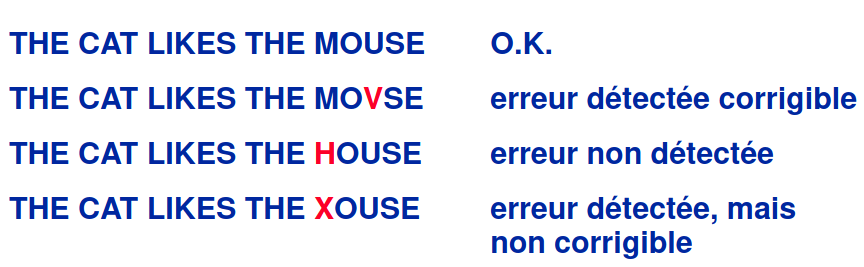
\includegraphics[width=0.7\textwidth]{img/Erreur2.png}
			\end{figure}
			
			\textbf{Ex3 : }Code a répétition
		
				Répété chaque bit envoyé 1 fois :
				\begin{itemize}
					\item 0 $\rightarrow$ 00
					\item 1 $\rightarrow$ 11
				\end{itemize}
				
				donc 00 et 11 sont correcter et 01 et 10 sont faux
				
			\textbf{Ex4 : }Code a double répétition
				Répété chaque bit envoyé 2 fois :
				\begin{itemize}
					\item 0 $\rightarrow$ 000
					\item 1 $\rightarrow$ 111
				\end{itemize}
				
				donc 000 et 111 sont correcte et 001, 010, 011, 100,101 et 110 sont faux
				
			\textbf{Ex5 :} Code de Hamming
				Code(15,11)
				
				i = 1 0 1 0 1 0 1 1 0 0 1
				
				On a :
				\begin{itemize}
					\item 11 bits entrée
					\item 15 bits codé $\rightarrow$ 4 bits de redondance/parité
				\end{itemize}
				
				On place les bits de codage au rangs de "puissance de 2" pour déterminer les 4 bits de rédondance
				
				\begin{tabular}{ccccccccccccccc}
					15 & 14 & 13 & 12 & 11 & 10 & 09 & 08 & 07 & 06 & 05 & 04 & 03 & 02 & 01\\
					1 & 0 & 1 & 0 & 1 & 0 & 1 & $c_4$ & 1 & 0 & 0 & $c_3$ & 1 & $c_2$ & $c_1$ 
				\end{tabular}
				
				Ensuite on prend les rangs avec un bit = 1
				
				\begin{tabular}{c|c}
				15 & 1 1 1 1\\\hline
				13 & 1 1 0 1\\\hline
				11 & 1 0 1 1\\\hline
				9  & 1 0 0 1\\\hline
				7  & 0 1 1 1\\\hline
				3  & 0 0 1 1
				
				\end{tabular}
				
				Ensuite on calcule le module 2 (en additionnant les valeurs de chaque colones d'avant avec 0 si paire et 1 si impaire)
				
				\begin{tabular}{cccc}
				1 & 1 & 1 & 1\\
				1 & 1 & 0 & 1\\
				1 & 0 & 1 & 1\\
				1 & 0 & 0 & 1\\
				0 & 1 & 1 & 1\\
				0 & 0 & 1 & 1\\ \hline
				0 & 1 & 0 & 0\\
				$c_4$ & $c_3$ & $c_2$ & $c_1$
				
				\end{tabular}
				
				On peut verifier  car seulement $c_3$ contient un 1 et est a la position 4 (0100)
				
				\begin{tabular}{cccc}
				1 & 1 & 1 & 1\\
				1 & 1 & 0 & 1\\
				1 & 0 & 1 & 1\\
				1 & 0 & 0 & 1\\
				0 & 1 & 1 & 1\\
				0 & 0 & 1 & 1\\ 
				\textcolor{green}{0} & \textcolor{green}{1} & \textcolor{green}{0} & \textcolor{green}{0}\\\hline
				\textcolor{red}{0} & \textcolor{red}{0} & \textcolor{red}{0} & \textcolor{red}{0}\\
				$c_4$ & $c_3$ & $c_2$ & $c_1$
				
				\end{tabular}
				
				Réception d'un message avec une erreur :
				
				\begin{tabular}{ccccccccccccccc}
					15 & 14 & 13 & 12 & 11 & 10 & 09 & 08 & 07 & 06 & 05 & 04 & 03 & 02 & 01\\
					1 & 0 & 1 & 0 & 1 & 0 & \textcolor{red}{0} & 0 & 1 & 0 & 0 & 0 & 1 & 0 & 0 
				\end{tabular}
				
				Et donc on fait comme avant et on calcule le modulo 2
				
				\begin{tabular}{cccc}
				1 & 1 & 1 & 1\\
				1 & 1 & 0 & 1\\
				1 & 0 & 1 & 1\\
				0 & 1 & 1 & 1\\
				0 & 1 & 0 & 0\\
				0 & 0 & 1 & 1\\ \hline
				\textcolor{red}{1} & \textcolor{red}{0} & \textcolor{red}{0} & \textcolor{red}{1}
				
				\end{tabular}
				
				Et donc \textcolor{red}{1} \textcolor{red}{0} \textcolor{red}{0} \textcolor{red}{1} = 9 donc le bit 9 est érroné
				
			\textbf{Avantage} :
			\begin{itemize}
				\item redondance minimale pour la capacité correctrie voulue a la taille du bloc voulue
				\item facile a réaliser
				\item Peut trouver une seule erreur dans le block (inconvénient)
			\end{itemize}
			
		\subsubsection{Codes et redondance}
			ajouter de la redondance = certains mots sont correct et d'autre incorrect
			
			Cela permet détection/correction. Si on a plus de redondance, on a plus de mots espacés et donc avoire de meilleur possibilités de detections/corrections et mais cela a un cout en débit a transmettre
			
		\subsubsection{Code VS. encodage}
			En fonction du code/dictionnaire ça va impacté sur les performances
			
			Choix de l'encodage  = Table d'entrée / sortie du codeur
			
			\begin{tabular}{|c|c|}
			\hline
			Input & Output\\ \hline
			000 & 000000 \\ \hline
			001 & 001111 \\ \hline
			010 & 010100 \\ \hline
			011 & 011101 \\ \hline
			\dots & \dots \\ \hline
			
			\end{tabular}
			
			Avec $k$ bits d'entrée et $n$ bit de sortie, on peut déterminer que :
			\begin{equation}
				\# \text{mots code} = n = 2^k
			\end{equation}
			
		\subsubsection{Théorie des codes}
		
			Comment ajouter de la redondance/définir le dictionnaire pour obtenir de bonnes capacité correctrices/détectrices en augmentant le débit de moins possible
			
			Distance de Hamming:
			
			Code($n,k$) Soit $k$ le nombre de bits utile et $n$ tel que $n-k$ est le nombre de bits de controle. Le \textbf{Taux du code} est $k/n$. On va choisir dans le dico le mots le plus proche trouvé en utilisant la distance. \textbf{code(n,k)} est de distance minimal $d$ détecte les erreurs d'ordre d-1 et corriges les erreurs d'ordre $\textit{floor[(d-1)/2]}$
			
			ex : 
			\begin{tabular}{c}
			0001101\\
			\textcolor{red}{1}001\textcolor{red}{0}01
			\end{tabular}Distance de 2
			
			ex2:
			
			\begin{tabular}{c}
			000OO\\
			11111
			\end{tabular} on a reçu 11010, d(00000,11010) = 3 et d(11111,11010) = 2 on choisis donc 11111
			
			
			TODO:A terminer